\documentclass{article}

\usepackage{graphicx} 
\usepackage{hyperref}                         % Pacchetti
\usepackage[italian]{babel}
\graphicspath{ {./images/} }
\usepackage{fancyhdr}
\usepackage{imakeidx}
\pagestyle{fancy}
\fancyhf{}
\fancyhead[LE,RO]{Istituto Tecnico Tecnologico “G. e M. Montani”}
\fancyfoot[CE,CO]{5°IN B a.s. 2021/2022}
\fancyfoot[LE,RO]{\thepage}
\usepackage{geometry}
\geometry{
	a4paper,
	total={210mm,297mm},
	left=40mm,
	right=40mm,
	top=20mm,
	bottom=20mm,
}

\makeindex[columns=1, title=Tavola dei contenuti, intoc]

\begin{document}
	
	
	\begin{titlepage}
		\begin{center}
			\huge\textbf{Montani WebSite}\\
			\Large\textbf{5 INB}\\
			\Large \textbf{Documento di Progettazione}\\
			\vspace{4cm}
			\large Project Manager: \textbf{Boussoufa Yacine}\\
			\large Data: \textbf{25/02/2022}\\
			\large Versione: \textbf{0.2}\\
			\large ID WP: \textbf{Allegato D}\\
			\large ID Progetto: \textbf{Montani}\\
			
		\end{center}
	\end{titlepage}
	
	\clearpage
	
	\begin{tabular}{ |p{1cm}|p{4cm}|p{3cm}|p{2cm}|  }
		\hline
		\multicolumn{4}{|c|}{Cronologia delle revisioni} \\
		\hline
		ID& Cambiamenti &Data di creazione&Autore\\
		\hline
		001   & Creazione    &08/02/2022&   Camilletti Samuele\\
		\hline
		002   & Modifiche e correzioni    &25/02/2022&   Camilletti Samuele\\
		\hline
	\end{tabular}
	
	\clearpage
	
	\tableofcontents
	\printindex	
	
   

    %_______________________________________________________________________________________________
    %ANALISI PROBLEMA	
	\section{\textbf{Introduzione al documento}}
	\flushleft
	\normalsize
	Il presente documento ha lo scopo di presentare l'analisi e la progettazione Front-End e Back-End del Sito Web sviluppato per l'attività di PCTO svolta nel mese di Febbraio 2022, dal gruppo composto da Boussoufa Yacine, Camilletti Samuele, Capretti Mattia e Nucci Enrique.
	\normalsize
	\subsection{\textbf{Commessa del cliente}} 
	\flushleft
	\normalsize
	L'Istituto Tecnico Tecnologico "G. e M. Montani" di Fermo ha incaricato, attraverso il committente Trasatti Daniele, il restyling grafico e funzionale del sito web scolastico, mirato a migliorare le modalità di usufruizione dei servizi scolastici dell'Istituto.
	 \subsection{\textbf{Obiettivo}} 
	\flushleft
	\normalsize
	L'obiettivo del presente progetto è di realizzare un sito web per l'Istituto Tecnico Tecnologico Montani di Fermo. La scuola dispone già di un sito web, il quale non rispetta i requisiti grafici e funzionali definiti dal modello standard di siti web scolastici realizzato dal Team per la Trasformazione Digitale su richiesta del Ministero dell'Istruzione. Il progetto si basa sulla metodologia, gli strumenti e il design fornito dal team di Designers Italia e a sua volta, contribuisce ad alimentare la conformità della Pubblica Amministrazione. Per ulteriori informazioni consultare \url{https://docs.italia.it/italia/designers-italia/design-scuole-docs/it/master/progetto-siti-web-delle-scuole.html}. Partendo dallo studio della realtà pre-esistente è stato necessario ridefinire le modalità di navigazione e di interfacciamento con l'utente nel sito web.

	\section{\textbf{Analisi}} 
	
    \subsection{\textbf{Analisi della realtà pre-esistente}}
    Come descritto negli allegati di Project Management (Allegato Gantt ...), è stato necessario compiere un'intensa attività di analisi preliminare per comprendere pienamente l'ambito del progetto.
	Il sito web del Montani utilizzato tra il 2016 e il 2022, è risultato inadeguato sotto diversi aspetti. In primo luogo, la grafica risulta incoerente  e non adeguata sia da un punto di vista estetico che da un punto di vista funzionale: il menù delle articolazioni è poco utilizzato e non mette in risalto la varietà dei percorsi di studio offerti; inoltre rende possibile l'accesso alle pagine delle articolazioni soltanto dal menù a tendina e non dalle sottopagine dedicate;\\
	Il menù laterale sinistro, con le diverse funzionalità, risulta confusionario e inaccessibile, per via della lunga lista di servizi offerti. In particolare da dispositivi mobili non è responsive e necessita lo scorrimento fino a fine pagina per permetterne la visualizzazione.\\
	L'header della pagina essendo un'immagine non presenta le caratteristiche di responsive ed accessibilità.
	Sono infine numerose le pagine del sito non funzionanti e non più aggiornate, le quali necessitano una completa revisione.
	Dopo un'attenta analisi della situazione attuale, si è deciso di prendere in considerazione il modello standard fornito dal Team per la Trasformazione Digitale e di utilizzarlo come tema base di partenza.
	La dimostrazione grafica del tema in questione è reperibile al link \url{http://design-italia.marcogargano.com/}.
	
	\subsection{\textbf{Piattaforma WordPress}}
	WordPress è una piattaforma software di content management system (CMS) che, operando lato server in un database, consente la creazione di un sito Internet formato da contenuti testuali o multimediali, gestibili ed aggiornabili in maniera dinamica; facendo uso di codice HTML CSS e JavaScript. Wordpress mette a disposizione anche plugin e temi per la personalizzazione del sito web. Wordpress necessita di un database per la memorizzazione di tutte le informazioni relative al sito e un Web Server Apache. Per la mantenimento del web server e del relativo database viene utilizzato il servizio hosting Aruba. Il dominio (istitutomontani.edu.it) segue le normative relative agli indirizzi istituzionali.	
	
	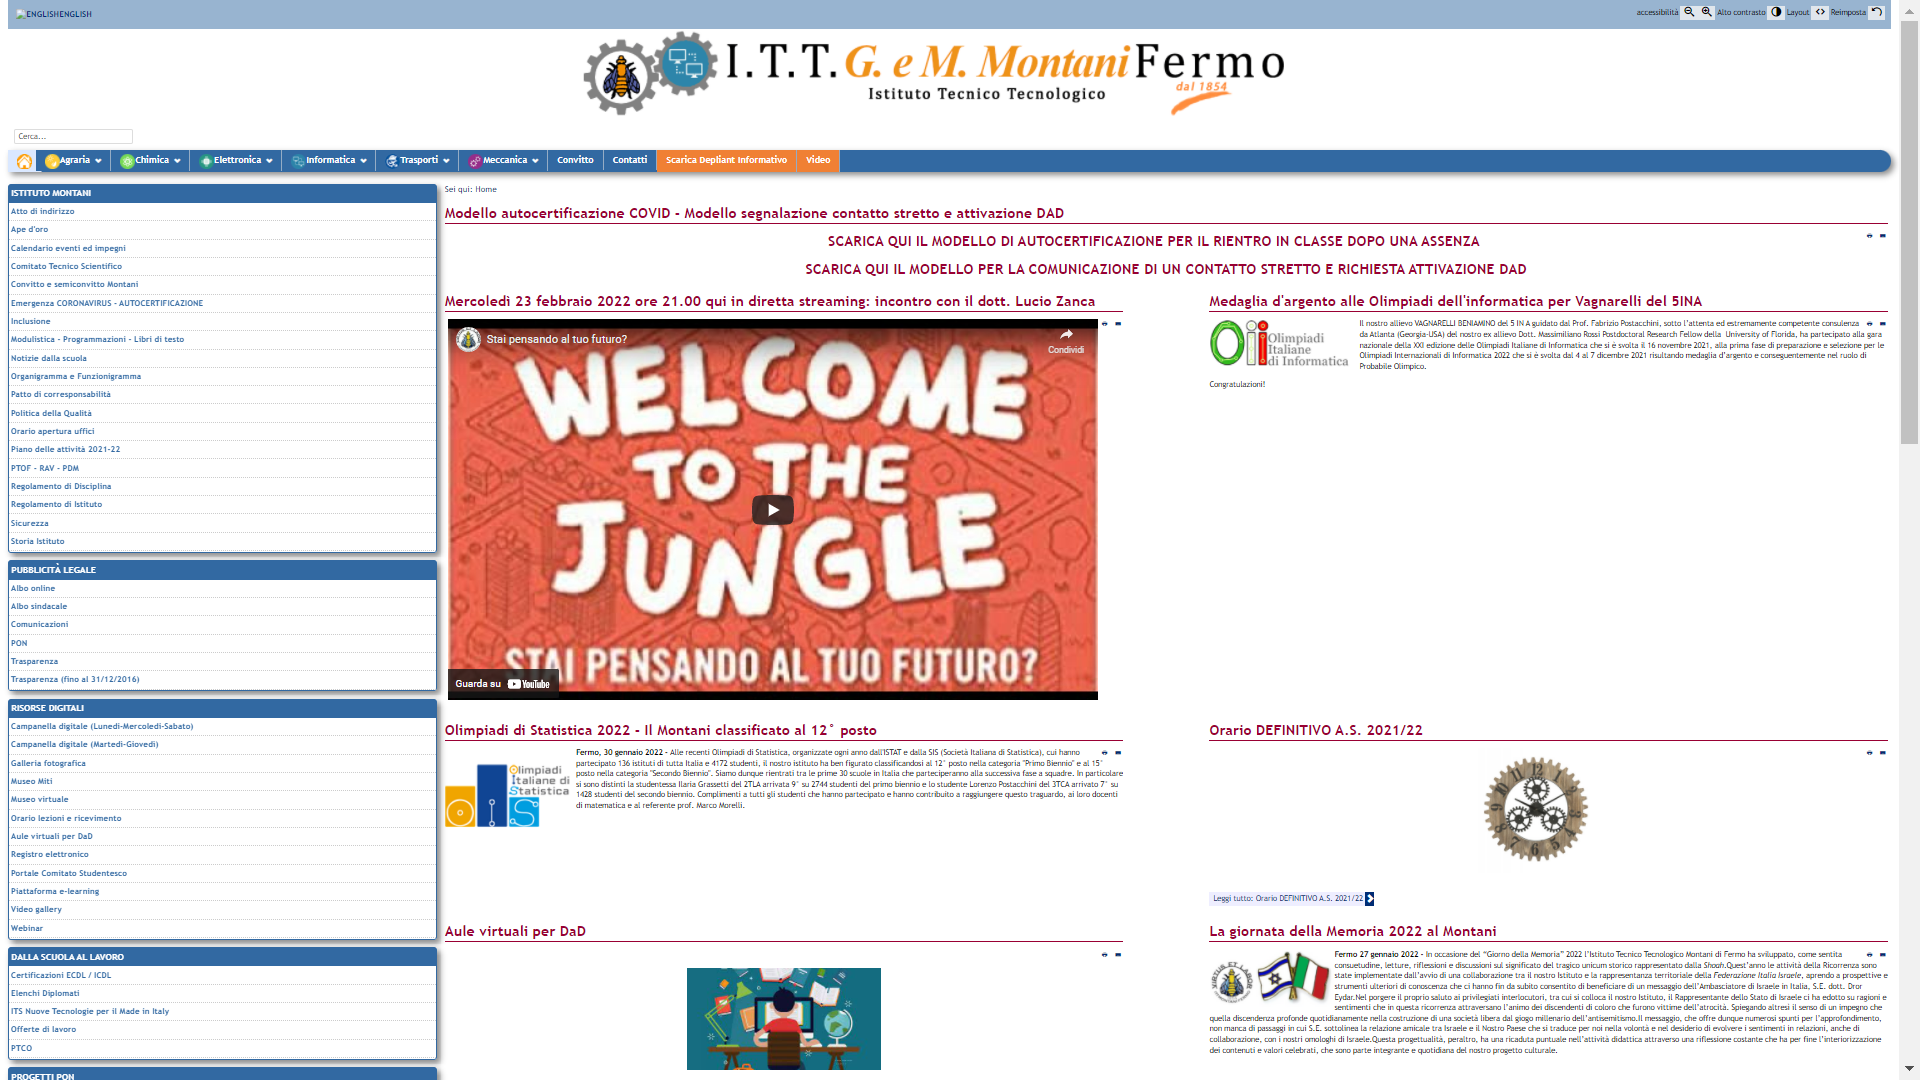
\includegraphics[scale=0.18]{ittmontaniex.png}
	\subsection{\textbf{Analisi e progettazione prototipo in WordPress}}
	Dopo un'attenta analisi dei requisiti funzionali e non funzionali descritti nel documento di Specifica dei Requisiti (Allegato A), si è deciso di utilizzare il CMS WordPress per la realizzazione di un prototipo grafico da mostrare al cliente, modificando il template istituzionale. 
	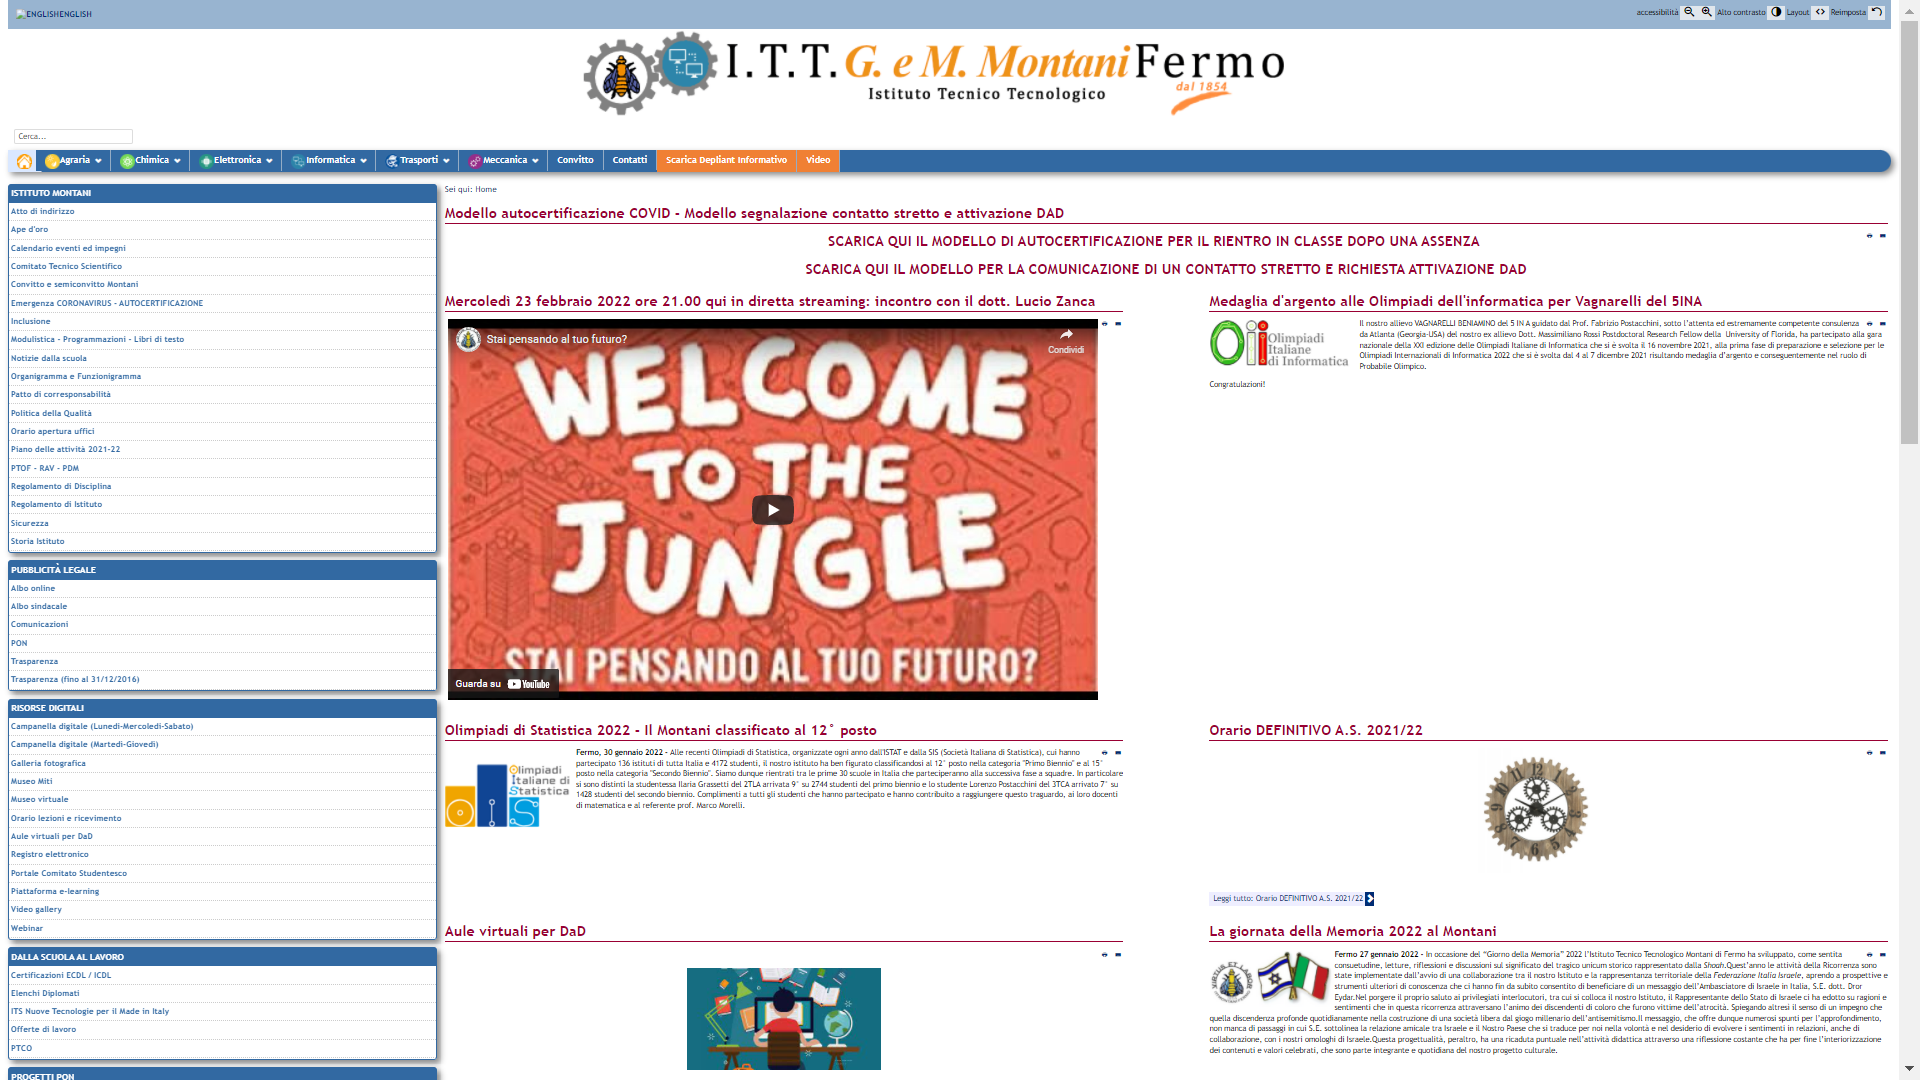
\includegraphics[scale=0.18]{ittmontaniex.png}
	Il prototipo grafico della home page è stato approvato ma sono state commissionati diverse revisioni, le quali sono state aggiunte al documento SRS. L'accordo finale raggiunto con il cliente prevede:
	\begin{itemize}
	    \item Un header rinnovato con un menù a tendina suddiviso per categoria di utente (le categorie di utente sono descritte nel documento di specifica dei requisiti).
	    \item Uno slider rappresentativo di tutte le articolazioni presenti nell'offerta formativa scolastica.
	    \item Uno slider di notizie principali da mantenere in costante aggiornamento.
	    \item Una sezione di notizie a blocchi affiancata dai principali servizi offerti dalla scuola.
	    \item Un footer descrittivo dei principali contatti scolastici.
	\end{itemize}
	In tutte le pagine del sito è stato deciso di inserire un banner grafico, inserito in aggiunta al CSS di base in modo da rendere più gradevole l'impatto grafico. \\
	Le notizie del sito sono state invece implementate attraverso gli articoli di WordPress.\\
	
	\subsection{\textbf{Diagramma Use-Case}}

	Un caso d’uso è una sequenza di transizioni in un sistema il cui compito è di conseguire un risultato di valore misurabile per un singolo attore del sistema.\\
    L’attore specifica un ruolo assunto da un utente o altre entità che interagisce con il sistema nell’ambito di un’unità di funzionamento.\\
    Lo scenario rappresenta le categorie di utenti che interagiscono con il sistema informativo, in particolare visitatore, studente, personale, segreteria ed amministratore.
	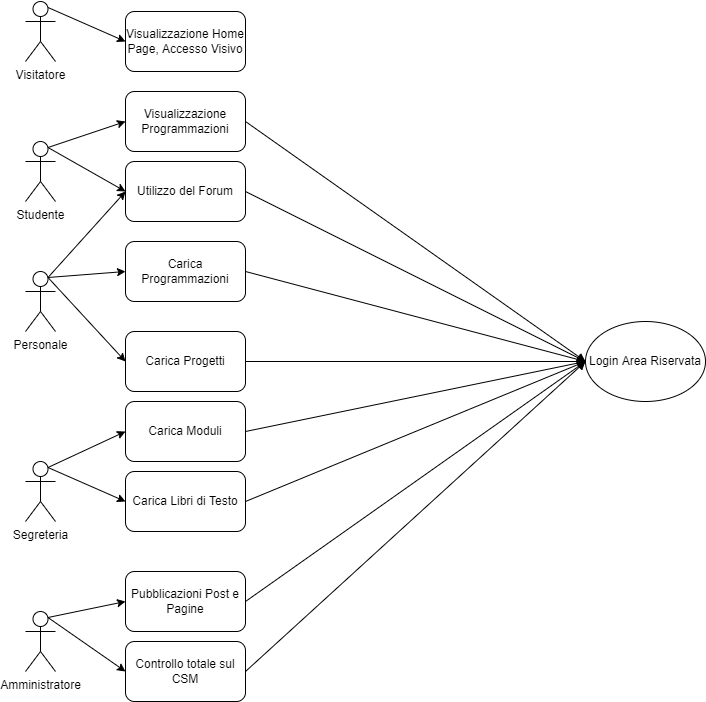
\includegraphics[scale=0.2]{usecase.drawio.png}
		
	\subsection{\textbf{Responsive}}

	Per implementare il requisito non funzionale relativo alla responsiveness del sito è stata sfruttata la caratteristica dei file CSS (Cascading Style Sheets) con i quali, aggiungendo una parte di codice dedicata alla visualizzazione su schermi di risoluzione differente, è stato possibile rendere portabile il sito.
	
	\subsection{\textbf{Forum}}

	Per implementare il requisito funzionale relativo al Forum è stato utilizzato un Plugin dedicato il quale gestisce contemporaneamente un'interfaccia Back-end e Front-end. Si è deciso di un utilizzare per un plugin per via della sua facile implementazione all'interno del Sito Web, considerando la portabilità dello stesso.\\
	Il forum è stato suddiviso in 2 gruppi, una parte dedicata ai Docenti e una parte dedicata agli Studenti. Le due categorie di utenti sono raggruppate in 2 User group dedicati implementati nel plugin, i quali gestiscono i permessi.\\
	%\includegraphics[scale=0.18]{forumhomepage.png}
	L'utente dopo aver effettuato l'accesso può inserito può inserire una discussione cliccando sul tasto Nuovo Topic.\\
	L'utente può visualizzare una discussione scegliendone una dall'elenco e può inserire un post nella discussione cliccando su Rispondi.\\
	\subsection{\textbf{Login Google}}

	Per implementare il requisito funzionale relativo al Login sono state analizzate 3 opzioni:
	\begin{itemize}
	    \item Login tramite SPID.
	    \item Login tramite Google.
	    \item Login tramite API Spaggiari.
	\end{itemize}
	Dopo aver studiato la fattibilità delle opzioni, l'accesso tramite Google è risultato il più accessibile e facile da implementare. Utilizzando la piattaforma di interfacciamento Google Cloud Platform, la quale consente ad una piattaforma istituzionale di aver accesso ad un API per il login. Il collegamento tra la piattaforma ufficiale Google e Login di WordPress è stato implementato attraverso un plugin di accesso (Google Login), il quale è stato configurato per accettare solo email istituzionali.\\
	Per differenziare le categorie di utente (studente, personale, segreteria e amministratore) sono state utilizzate i ruoli di WordPress. Agli studenti viene automaticamente assegnato il ruolo Sottoscrittore, ai docenti il ruolo Contributore, alla segreteria il ruolo Editore e il ruolo Amministratore per il gestore del sito. L'assegnazione dei permessi è stata implementata attraverso una funzione 'hook' collegata alla registrazione di WordPress, la quale legge un file contenente le email istituzionali dei docenti e assegna di conseguenza i permessi.\\   
	
	
	\subsection{\textbf{Progettazione lato Back-end}}
	La seguente progettazione illustra il lato Front-End e Back-end del sito e il rapporto dei soggetti coinvolti con esso.	
	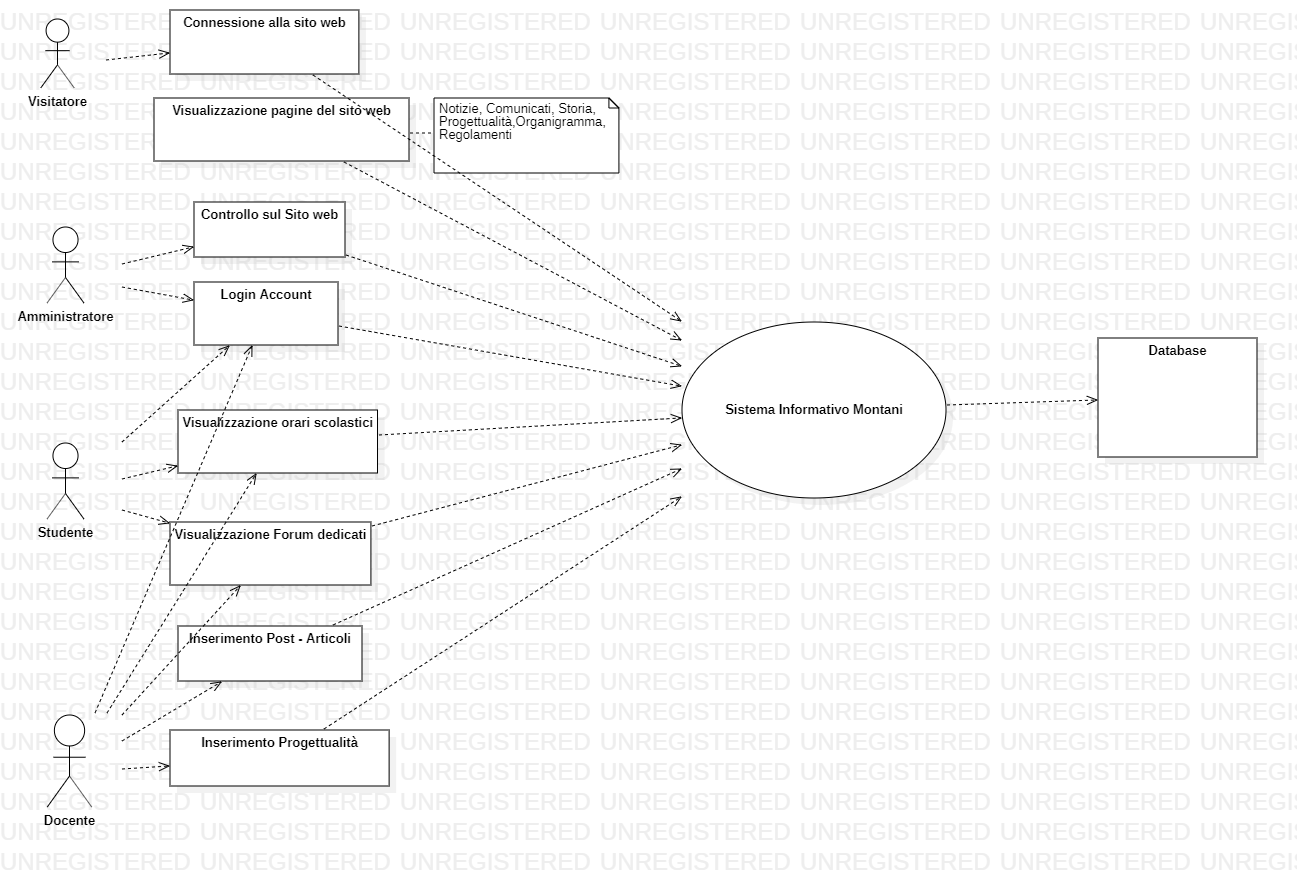
\includegraphics[scale=0.35]{UseCaseDiagram.png}
	\subsubsection{\textbf{Analisi Database}}
	Per soddisfare i requisiti RF-005,RF-009 e RF-010 relativi al documento della Specifica dei Requisiti, è stato necessario progettare un ampliamento del Database preesistente di Wordpress al fine di consentire una gestione della repository efficiente nella medesima base di dati.
	In particolare, si intende gestire i dati relativi alla modulistica, libri di testo scolastici, progettualità e programmazioni scolastiche.
	Per modulistica scolastica si intende la raccolta di documenti utilizzabili dai soggetti che frequentano l'Istituto per richiedere o effettuare una procedura. I file sono caricati dalla Segreteria scolastica e sono messi a disposizione per tutti gli utenti coinvolti nel sistema. I moduli sono suddivisi per categoria di utente: alunni e famiglie, docenti, pubblico e personale ATA.
	La modulistica scolastica è definita da un link di download per un file .doc/.pdf caricato nell'archivio Wordpress, una data di caricamento, dimensione del file e il nome dell'autore.
	Per libri di testo scolastici si intende un file contenente le informazioni relative ai libri adottati dal docente, per una specifica classe dell'Istituto. I libri pubblicati dalla Segreteria scolastica sono visibili da tutti gli utenti del sistema; è da notare infatti che le classi prime non possedendo un indirizzo istituzionale non potrebbero visualizzare i testi scolastici senza aver effettuato l'accesso.
	I libri di testo scolastici sono suddivisi per anno scolastico e anno di corso(PRIME, SECONDE...) come nella versione precedente della repository e conterranno un link di download al relativo .pdf caricato nell'archivio. L'entità libro di testo conterrà inoltre una data di caricamento, la dimensione del file, il nome dell'autore e la rispettiva classe.
	I docenti e il committente hanno inoltre evidenziato la necessità di implementare un'ulteriore repository dedicata alle progettualità svolte nel corso degli anni.
	Un progetto si compone di un nome progetto, un obiettivo, una tipologia progetto (PCTO, Scuola e Territorio,...), una descrizione progetto, eventuali foto allegate, una data di realizzazione, il team di sviluppo e relativo file di progetto. I progetti sono inoltre caratterizzati da un Anno Scolastico, una classe e dalla relativa Articolazione.\\ 
	Per identificare univocamente un progetto si è scelto di utilizzare il nome progetto, in quanto non è opportuno, anche per motivi di diritto di autore, che esistano 2 progetti con lo stesso nome.
	Per associare le foto ad un progetto è stata definita un'entità foto la quale contiene le informazioni relative al percorso del file, ed è stato posto un limite ad un massimo di 3 foto per progetto.
	I progetti sono caricati dai docenti dell'Istituto e sono visibili a tutte le categorie di utenza, al fine di accrescere il lavoro svolto dagli studenti.\\
	Infine, è stato richiesto di implementare una repository dedicate alle programmazioni scolastiche svolte durante l'anno dalle singole classi dell'Istituto.
	Le programmazioni sono costituite da un link per il download di un file .pdf caricato nell'archivio, una data di caricamento, dimensione del file nome dell'autore, la classe, la materia e il relativo Anno Scolastico. Non sarà implementata un'entità materia, in quanto è impossibile fisicamente tenere traccia di tutte le materie e della loro evoluzione nel tempo.
	Le programmazioni, come per i progetti, possono essere caricati da utenti con permessi Docente.
	Le programmazioni possono essere visualizzate solo dagli utenti che hanno effettuato l'accesso al sistema.
	Un docente può caricare più progetti e più programmazioni. La segreteria può caricare più moduli e più libri di testo.
	Per identificare un account nel sistema si utilizza la progettazione fisica preesistente del database Wordpress, la quale memorizza gli account registrati in una tabella dedicata. 
	Come già specificato, i progetti, le programmazioni e i libri di testo saranno inoltre associati a una classe dell'Istituto. Una classe dell'Istituto sarà identificata da un'identificativo, una denominazione, un'anno di corso e l'anno scolastico corrente. Un anno scolastico identificherà univocamente i progetti, programmazioni e libri di testo nel tempo. La classe sarà inoltre associata ad un anno di corso (prime, seconde, terze, quarte, quinte). Su richiesta del committente la classe non sarà associata ad un anno scolastico, ma verrà riutilizzata nel corso degli anni, considerando che saranno i singoli documenti ad essere associati a un fattore temporale. 
	\subsubsection{\textbf{Inviduazioni delle entità}}
	\textit{Dalla realtà analizzata si descrivono le seguenti entit`a con i relativi attributi:}
    L'entità LibriTesto conterrà le informazioni relative ad un file memorizzato nell'archivio. Per la chiave primaria sarà utilizzato un intero incrementale più efficiente e immediato di una chiave composta. \\
	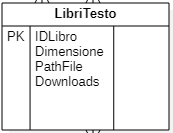
\includegraphics[scale=0.5]{libro.png}\\
    L'entità AnnoScolastico conterrà l'anno scolastico sotto forma di stringa e costituirà la chiave primaria. \\
	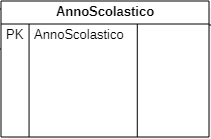
\includegraphics[scale=0.5]{annoscolastico.png}\\
    L'entità Articolazione conterrà la denominazione dell'articolo e costituirà la chiave primaria. Questa scelta è stata presa in quanto semplifica la gestione delle query nella ricerca dei progetti nelle pagine WordPress.\\  
	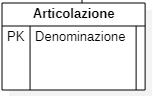
\includegraphics[scale=0.5]{articolazione.png}\\
    L'entità Classe conterrà la sezione della classe, l'anno del corso. La sezione della classe costuitirà la chiave primaria in quanto non esistono più classi con lo stessa denominazione. \\
	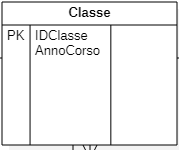
\includegraphics[scale=0.5]{classe.png}\\
    L'entità Modulistica conterrà la informazioni relative al modulo archiviato nel database. Per la chiave primaria sarà utilizzato un intero incrementale.\\
	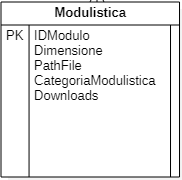
\includegraphics[scale=0.5]{modulistica.png}\\
    L'entità Programmazione conterrà la informazioni relative ad una programmazione archiviata nel database. Per la chiave primaria sarà utilizzato un intero incrementale.\\
	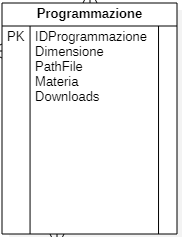
\includegraphics[scale=0.5]{programmazione.png}\\
    L'entità Progetto conterrà la informazioni relative ad un progetto archiviato nel database. Per la chiave primaria sarà utilizzato il nome progetto in quanto non devono esistere due progetti con lo stesso nome.\\
	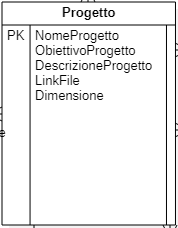
\includegraphics[scale=0.5]{progetto.png}\\
   L'entità Foto conterrà la informazioni relative ad una foto archiviata nel database. Sarà utile per associare più foto ad un progetto. Per la chiave primaria sarà utilizzato un intero incrementale.\\
	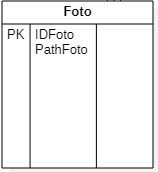
\includegraphics[scale=0.5]{foto.png}\\
   L'entità tipoProgetto conterrà la informazioni relative ad un tipo del progetto (Scolastico, PON, PCTO.. etc). Sarà utile per associare una tipologia ad un progetto. Per la chiave primaria sarà utilizzato un intero incrementale.\\
	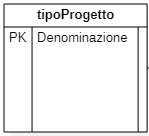
\includegraphics[scale=0.5]{tipoprogetto.png}
	\subsubsection{\textbf{Individuazioni delle associazioni}}
	Dalla realtà analizzata si individuano le seguenti associazioni:\\
	Tra AnnoScolastico e LibriTesto esiste l’associazione essere utilizzati:\\
	Un file di Libri di Testo deve essere utilizzato in un Anno Scolastico.\\
	In un Anno Scolastico devono essere utilizzati più Libri di Testo.\\
	\vspace{2mm}
	Tra AnnoScolastico e Progetto esiste l’associazione essere effettuato:\\
	Un progetto deve essere effettuato in un Anno Scolastico.\\
	In un Anno Scolastico possono essere effettuati più Progetti.\\
	\vspace{2mm}
	Tra AnnoScolastico e Programmazione esiste l’associazione essere conseguita:\\
	Una Programmazione deve essere conseguita in un Anno Scolastico.\\
	In un Anno Scolastico possono essere conseguite più Programmazioni.\\
	\vspace{2mm}
	Tra Classe e Programmazione esiste l’associazione svolgere:\\
	Una Programmazione deve essere svolta da una Classe.\\
	Una Classe deve svolgere più Programmazioni.\\
	\vspace{2mm}
	Tra Classe e LibriTesto esiste l’associazione adoperare:\\
	Un file di Libri di Testo deve essere adoperato da una Classe.\\
	Una Classe deve adoperare più file di Libri di Testo.\\
	\vspace{2mm}
	Tra Classe e Progetto esiste l’associazione effettuare:\\
	Un Progetto deve essere effettuato da una Classe.\\
	Una Classe può effettuare più Progetti.\\
	\vspace{2mm}
	Tra Classe e Articolazione esiste l’associazione appartenere:\\
	Una Classe deve appartenere a una Articolazione.\\
	Una Articolazione deve appartenere a più Classi.\\
	\vspace{2mm}
	Tra tipoProgetto e Progetto esiste l’associazione caratterizzare:\\
	Una Progetto deve essere caratterizzato da un tipo Progetto.\\
	Una tipo di Progetto può caratterizzare più Progetti.\\
	\vspace{2mm}
	Tra Foto e Progetto esiste l’associazione allegare:\\
	Una Progetto può allegare più Foto.\\
	Una Foto deve essere allegata a un Progetto.\\
	\subsubsection{\textbf{Modello E/R}}
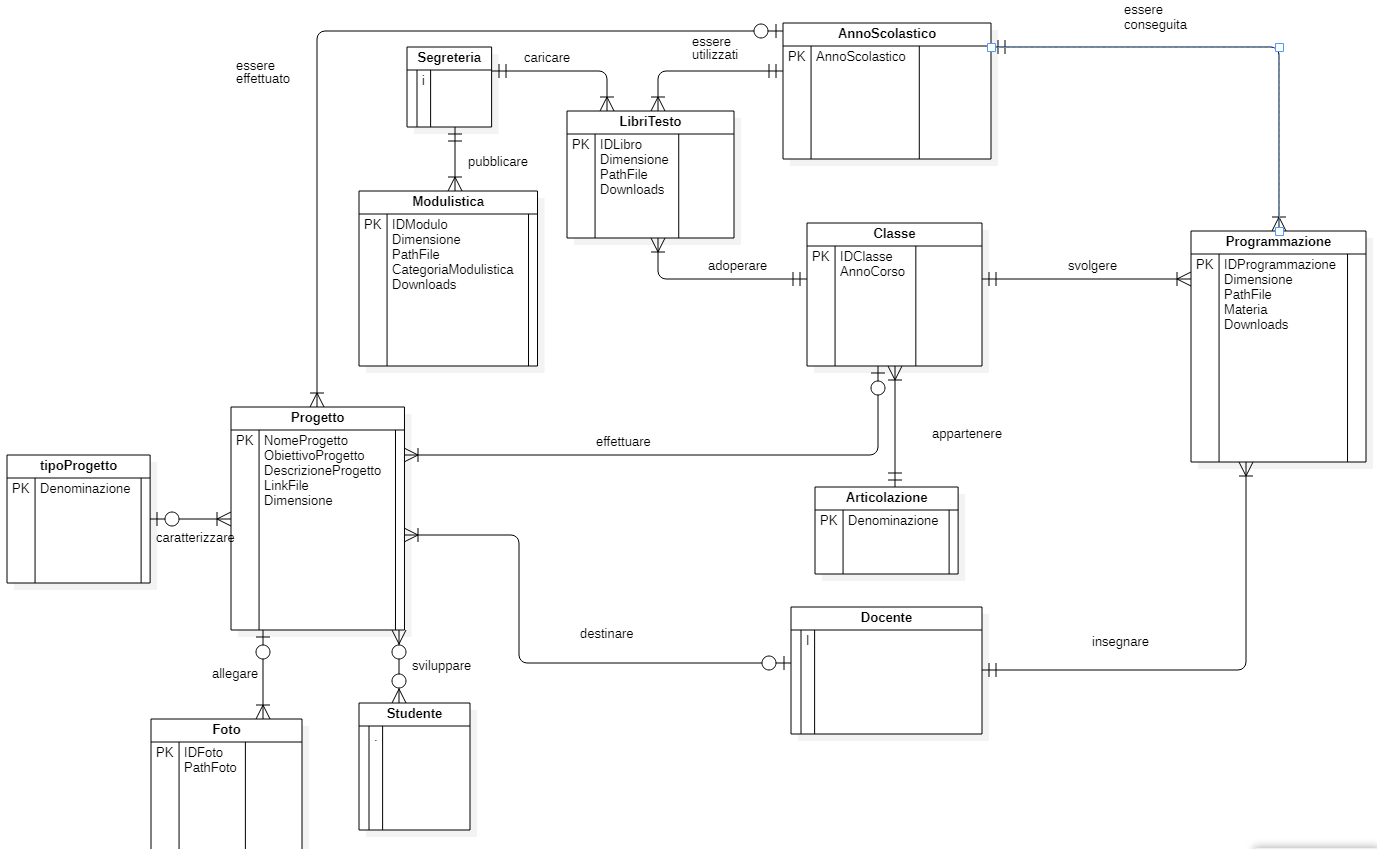
\includegraphics[scale=0.4]{modelloer.png}
	\subsubsection{\textbf{Modello logico}}
	%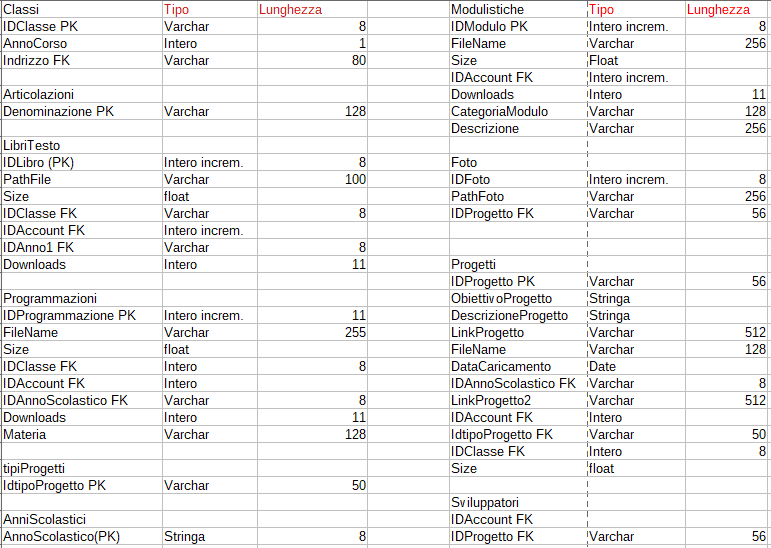
\includegraphics[scale=0.5]{modellologico.png}
	\subsubsection{\textbf{Modello fisico}}
%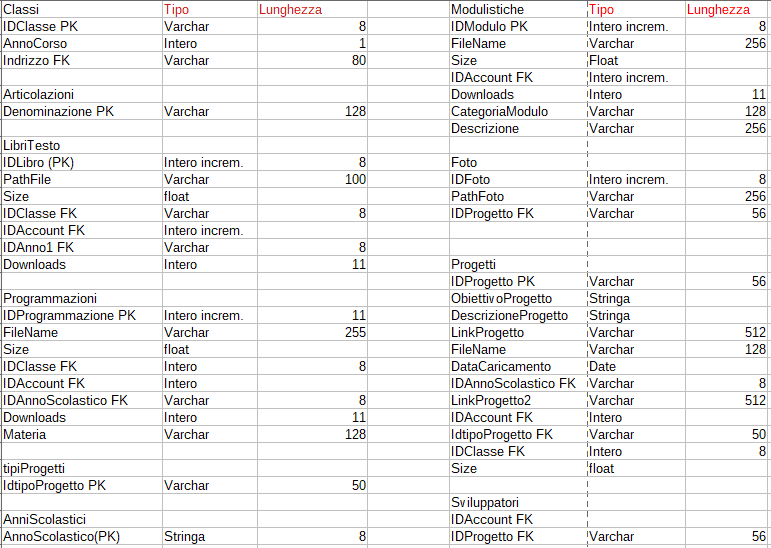
\includegraphics[scale=0.5]{modellologico.png}
	\subsection{\textbf{Browser supportati}}
	Il sito web è accessibile da qualsiasi device connesso ad internet, attraverso l'utilizzo di un browser web e digitando l'indirizzo istitutomontani.edu.it.\\
	Al caricamento della pagina verrà mostrata l'homepage, dalla quale si potrà scegliere il facilmente il servizio che l'utente sta cercando. 
	
	\subsection{\textbf{Ottimizzazioni al motore di ricerca}}
	SEO, ....	
\clearpage
	
\section{\textbf{Ulteriori specifiche}}
Ulteriori specifiche, se necessarie, verranno aggiunte nelle prossime versioni del seguente documento.
\end{document}
	
    